\documentclass{beamer}

\usepackage{multirow}

\AtBeginSection[]
{
  \begin{frame}
    \frametitle{Table of Contents}
    \tableofcontents[currentsection]
  \end{frame}
}

\title{Modeling Zombies and Infection}
\author{Ricky Marske and Steven Rosendahl}
\date{}

\usetheme{metropolis}

\begin{document}

\frame{\titlepage}

\section{A Simple Model}

\begin{frame}{Population Decay}
\begin{itemize}
\item Population decay can be modeled by
\[y=a(1-r)^{x}\]
\pause
\item $a:$ Initial amount of population
\pause
\item $r:$ Decay rate
\pause
\item $x:$ The amount of time that has passed
\end{itemize}
\end{frame}

\section{Adding Complexity}

\begin{frame}{Probability}
\begin{itemize}
\item In the initial model, we assumed
\pause
\begin{enumerate}
\item No one was immune
\pause
\item Non-Infected would have no response to infected
\pause
\item No one could survive the virus or be cured
\end{enumerate}
\end{itemize}
\end{frame}

\begin{frame}{Immunities}

\end{frame}

\begin{frame}{Non-Infected Responses}

\end{frame}

\begin{frame}{Cures and Survival}
\begin{itemize}
\item The time at which a cure is introduced affects the model
\pause
\item Can be represented by a wave equation:
\[
u_{tt}-k^{2}u_{xx}=0
\]
\pause
\item To show the offset, we have
\[
u_{tt}-k^{2}u_{xx}=\zeta
\]
\pause
\item $\zeta$ represents the time offset
\pause
\item This yields the solution
\[
u(x,t)=\zeta+\sum_{n=1}^{\infty}(k_{1}\sin{t}+k_{2}\cos{t})\sin{n\pi x}
\]
\end{itemize}
\end{frame}

\begin{frame}{Cures and Survival}
\begin{center}

\begin{minipage}{0.4\textwidth}
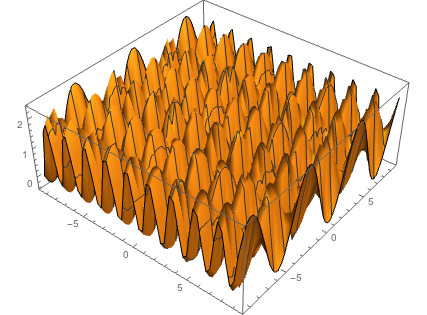
\includegraphics[scale=0.3]{cure_01}\\
$n=1$
\end{minipage}
\begin{minipage}{0.4\textwidth}
\pause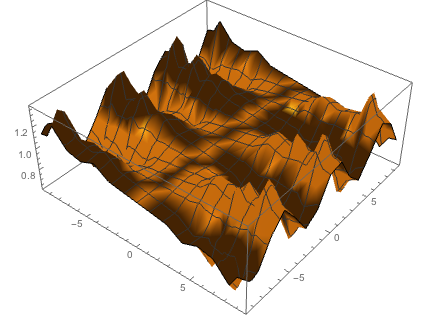
\includegraphics[scale=0.3]{cure_02}\\
$n=100$
\end{minipage}

\begin{minipage}{0.4\textwidth}
\pause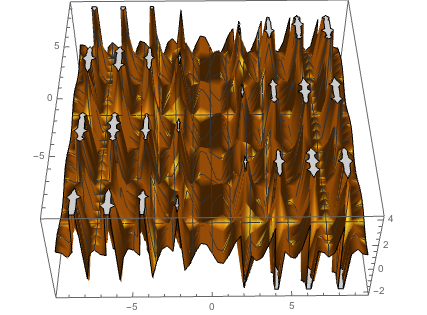
\includegraphics[scale=0.3]{cure_0201}\\
$n=500$
\end{minipage}
\begin{minipage}{0.4\textwidth}
\pause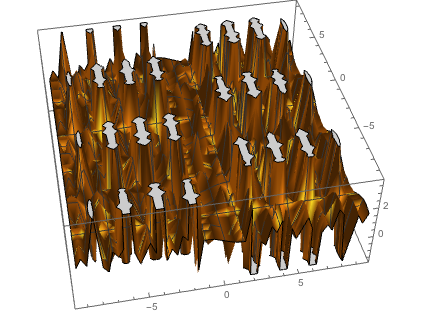
\includegraphics[scale=0.3]{cure_03}\\
$n=1000$
\end{minipage}

\end{center}
\end{frame}

\begin{frame}{Cures and Survival}
\[
u(x,t)=\zeta+\sum_{n=1}^{\infty}(k_{1}\sin{t}+k_{2}\cos{t})\sin{n\pi x}
\]
\begin{itemize}
\item There is a saddle regardless of $\zeta$
\pause
\item The system will move towards the saddle no matter what
\end{itemize}
\end{frame}

\section{Modeling Outside of NetLogo}

\end{document}
